\section{Software implementation}

\subsection{Autopilot}
The Autopilot is mad up of 2 separate PID loops, to implement PID loops the MiniPID library was used\cite{minipid}. It allows for setting output limits, which setup in the constructor of the Autopilot as seen in listing~\ref{lst:autopilot_con}. It can also be seen that the PID terms are all set to -1, this is used to indicate an invalid valued. There is only one set of PID terms because terms for the thruster was not parameterized out to the website. Therefore some relaxed values are set, so the motor is not going to accelerate to much. 

\begin{lstlisting}[caption = {Constructor method of the Autopilot}, captionpos=b, label={lst:autopilot_con}, language=C++,firstnumber=1]
Autopilot::Autopilot(IPositionMotor& rudder, ISpeedMotor& thruster): rudder_pid_(0, 0, 0), thruster_pid_(1,0,0), rudder_(rudder), thruster_(thruster)
{
	max_speed_ = 10; //in km/h
	p_ = -1; //Invalid value
	i_ = -1; //Invalid value
	d_ = -1; //Invalid value
	thruster_pid_.setOutputLimits(0, 20); //Hardcoding limits, maybe this should be done through the user interface
	rudder_pid_.setOutputLimits(48, 76);  //A servo has diffuculties at the edges ei. 0 and 90 so it is limited

	thruster_pid_.setPID(0.01,0,0);

}
\end{lstlisting}

The Autopilot works by setting the rudder and thruster PWM outputs from a calculation done by the MiniPID library. For the rudder the the setpoint is always 0, since the navigation outputs what direction to steer. The thruster has a setpoint of the max speed set in the constructor, and it also gets it's error from the navigation. The navigation calls the \texttt{Run} function in the autopilot with a NMEA telegram, the autopilot can parse either a APB or a VTG telegram. The APB telegram includes the direction to steer, and the VTG holds current speed of the boat. 

It was decided that stopping the boat just means to stop the motor and center the rudder. 

Before the \texttt{Run} function will work, there needs to have been a call to the \texttt{SetParameters} function, which sets the rudder PID terms. 

\subsection{JSONReceiver}
The responsibility of the JSONReciever is to get the activeParam.JSON, and the toNav.JSON files and parse them. After parsing it needs to call the appropriate functions in other object to let them know of this new data. To handle the JSON format in c++ the "json for modern c++" library by Niels Lohmann was used\cite{json}. 

The recieving of toNav.json works by reading the contents of file, and parsing it into JSON, after this it needs to figure out what kind of task is in the file. This is done by first using the json find function on the parsed json object. If the task is either; none, stop, start, just the task is passed on to the Navigation via the PerformTask function. If the task is calcCoverage, it goes through and checks if the toNav protocol is adhered to. If every thing is good it create a CoverageRectangle object which is then passed on to the Navigation together with the task, through the PerformTask function.
The exact same thing happens with the calcP2P task, but it creates a TargetPosition object instead.

To receive the active parameter profile the JSONReciever, parses the activeParam.json file with the "json for modern c++" library like before. Then it reads all the information and assigns it to the proper variables, so it can send to the Navigation and Autopilot, through the SetParameters function in both of them.

\subsection{Servo}
The Servo class has responsibility of controlling any kind of servo via a GPIO pin. To set the position of the motor it takes a position described as a percentage ei. a double between 0-100. To move a servo from one extremity to the other, it does not require a duty-cycle from 0-100, but instead a period lenght between 500 µs and 2500 µs\cite{pigpio}. Therefore the percentage needs to be converted and this is done in the helper function \texttt{percentageToServo} as seen in listing~\ref{lst:percent2servo}. To set the GPIO pin to the correct period the \texttt{GpioServo} function is used, which is a wrapper function for the pigpio library\cite{pigpio}.

\begin{lstlisting}[caption = {Percentage to servo periode convertion function}, captionpos=b, label={lst:percent2servo}, language=C++,firstnumber=1]
//Coverts a percentage into the right value for the servo
unsigned Servo::percentageToServo(const double percentage) const
{
	//Starts servo pulses on the GPIO, 0 (off), 500 (most anti-clockwise) to 2500 (most clockwise). 
	double x = 500 + percentage / 100 * (2000); 
	return static_cast<unsigned>(x);
}
\end{lstlisting}

\subsection{Ublox-neo7m}
The Ublox-neo7m is a GPS receiver by ublox, and it follows the NMEA protocol. This means that it sends out a serial telegram. To get this telegram from a serial device the simpleSerial library is used\cite{simple_serial}. The Ublox class has to responsibilities, it needs to get the concrete gps data, and then it needs to allow other classes to get pose data, speed, and status data. 

To make sure that this class is never blocking the execution of other functions by waiting for GPS data. It has the Setup function which returns a thread that runs the function getGPSData. This function keeps reading from the serial device, and when it gets a GGA telegram it parses it in to a Pose, and a bunch of variables needed for a GPSStatus object. It also parses the VTG telegram since it contains the speed of the GPSReciever. 

The GPS receiver outputs the latitude and longitude in a different format then what the rest of the system uses, there for it is converted with a helper function \texttt{convert\-Degree\-Minutes\-2\-Degrees}. To convert from \texttt{ddmm.mmmm} the format the rest of the system is using, this formula can be used \texttt{ddd + mm.mmmm/60}\cite{convertion}. The implementation of this formula can be seen in listing~\ref{lst:convertion}.


\begin{lstlisting}[caption = {Convertion between latitude longitude formats}, captionpos=b, label={lst:convertion}, language=C++,firstnumber=1]
double Ublox_neo7m::convertDegreeMinutes2Degrees(std::string degree_minutes) const
{
	//Find the . to be used as a fixed point
	const int delimtIndex = degree_minutes.find(".");
	
	//Extract ddd from start of string on til 2 before the .
	int ddd;
	try
	{
		ddd = std::stoi(degree_minutes.substr(0, delimtIndex - 2));
	}
	catch (...)
	{
		ddd = 0;
	}
	
	//The rest is mm
	double mm;
	try
	{
		mm = std::stod(degree_minutes.substr(delimtIndex - 2, degree_minutes.length() - 1));
	}
	catch (...)
	{
		mm = 0;
	}
	
	//return the convertion
	return ddd + mm / 60;
}
\end{lstlisting}

\subsection{User interface}
To develop the user interface for the project it was decided that to get the most flexibility it should be made as a website. To design the website the Bootstrap toolkit \cite{bootstrap}. This allows an easy creation of a simple design.
The design is build up of a simple side menu, with a logo and the menu items. Beside the menu is the context of the active menu. In figure~\ref{fig:frontpage} the active page is the front page.

\begin{figure}[H]
\centering
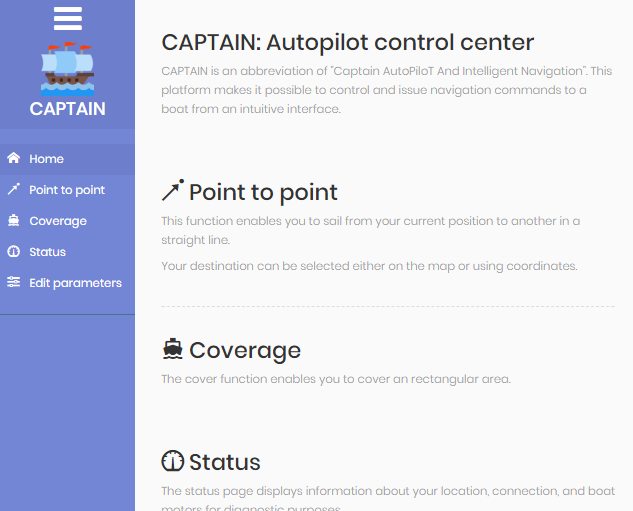
\includegraphics[width=0.7\linewidth]{Images/Implementation/frontpage}
\caption{Website front page}
\label{fig:frontpage}
\end{figure}

In figure~\ref{fig:p2ppage} it can be seen how the website handles categorization of functionality. In the figure there is a Coordinate panel which hold two more fields, one for latitude and longitude. Also there is a panel with the Estimated time en-route, and buttons to control the boat. The coordinate panel and Controls panel are also encapsulated in a box, which is besides a box with a map panel in it. This structure is created to make the website more size flexible, and it clearly defines different areas of interest.

\begin{figure}[H]
\centering
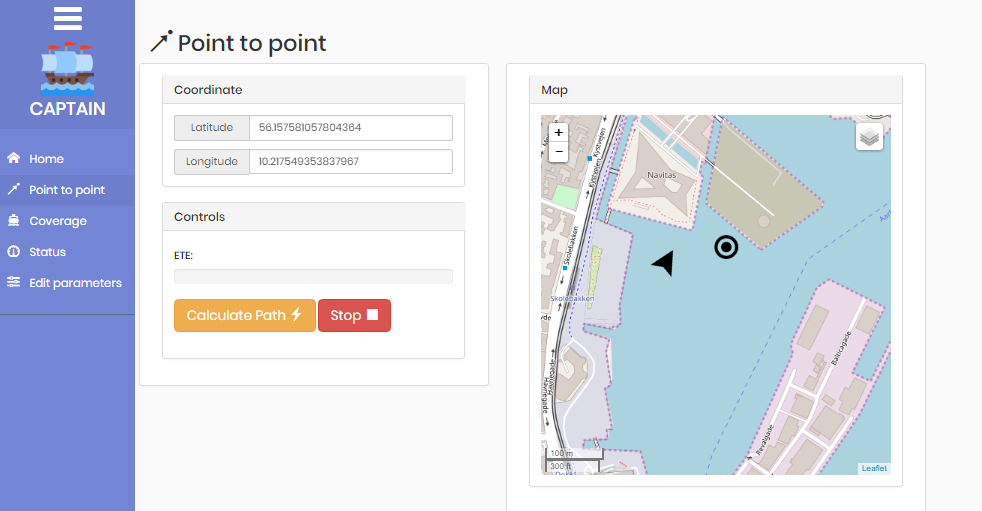
\includegraphics[width=0.9\linewidth]{Images/Implementation/p2p_page}
\caption{Website Point to point page}
\label{fig:p2ppage}
\end{figure}

Apart for the design of the website, it is develop with AngularJS\cite{angular}, which is a javascript framework. It makes data binding very easy, also it allows the website to only load once, after this the context is just changed. This context changing makes it very easy to develop different parts of the website separately, and still retain no loading of pages.

\subsubsection{Edit parameters}
The edit parameters page need to be able to create, delete, edit and active parameter profiles. A Parameter profile is a JSON object containing different parameters, it is the same as the active parameter profile, which is describe in the section~\ref{sec:active_param}.

A list of all of these parameter profiles is first loaded into a variable, if there are any. These parameter profiles comes from a file called profiles.JSON. When the user clicks the "New" button it create a default profile and pushes it to the list of profiles, and subsequently saves the list to the profiles.JSON file, as seen in listing~\ref{lst:newprofile}. 

\begin{lstlisting}[caption = {NewProfile function in editParam.js}, captionpos=b, label={lst:newprofile}, language=C++,firstnumber=1]
 $scope.NewProfile = function() {
    //Creates a new default profile and appends it to the list of Profiles_
    $scope.Profiles_.push({
      name_: "New Profile",
      parameter_names_: [
        "P", "I", "D", "Tool Width"
      ],
      parameters_: [
        0, 0, 0, 0
      ],
      creation_timestamp_: Date.now()
    });
    saveToFile("profiles", $scope.Profile_data_); //Sending the content to the server to get saved.
    $scope.Selected_profile_ = $scope.Profiles_[($scope.Profiles_).length - 1]; // Selects the new profile in the ui
  }
\end{lstlisting}

If the user presses the "Delete" button with a parameter profile selected, it will get deleted if there is not currently a profile open in the editor. If the profile being deleted is the active on, then the active one is replaces with an empty profile called None. When the profile is deleted from the list, then the list is saved to the profiles.JSON file, the source code can be seen in listing~\ref{lst:deleteprofile}

\begin{lstlisting}[caption = {DeleteProfile function in editParam.js}, captionpos=b, label={lst:deleteprofile}, language=C++,firstnumber=1]
 $scope.DeleteProfile = function(index) {
     if ($scope.Editing_profile_ != true) { //Checks to make sure you are not deleting the profile that's currently being edited
 
 		if($scope.Profiles_[index] == $scope.Active_profile_ ){
 			$scope.Active_profile_ = {
 		      name_: "None",
 		      creation_timestamp_: Date.now()
 		    }
 			saveToFile("active", $scope.Active_profile_);
 		}
 
 	  $scope.Profiles_.splice(index, 1) //Removes one element from the list at index
 
       if (index < 1) {
         $scope.Selected_profile_ = $scope.Profiles_[0];
       } else {
         $scope.Selected_profile_ = $scope.Profiles_[index - 1]; //Selects the profile under the one deleted.
       }
 
       saveToFile("profiles", $scope.Profile_data_); //Sending the content to the server to get saved.
     } else {
 
     }
   }
\end{lstlisting}

Pressing the "Edit" button changes a boolean that reveals a edit section. Two variables are updated first the \texttt{Profile\_} is updated with the values of the profile selected in the list of profiles. After this the \texttt{Profile_} is copied in to the \texttt{Revert\_profile\_}, this makes sure that the staring values are kept track of, if the user at a later point wants to revert. The exact sequence of the EditProfile function can be seen in listing~\ref{lst:editprofile}.

\begin{lstlisting}[caption = {EditProfile function in editParam.js}, captionpos=b, label={lst:editprofile}, language=C++,firstnumber=1]
$scope.EditProfile = function(index) {
    if ($scope.Editing_profile_ != true && ($scope.Profiles_).length > 0) { //Makes sure that there is something to edit!
      $scope.Revert_profile_ = {}; //Makes sure a Revet_profile_ exists
      $scope.Profile_ = $scope.Profiles_[index];
      angular.copy($scope.Profile_, $scope.Revert_profile_); //Creates a copy of Profile_ into Revert_profile_ instead of reference
      $scope.Editing_profile_ = true; //turns on the panel in the ui.
    }
  }
\end{lstlisting}

When the edit section is visible the user can change any of the variables, when happy with the changes the user can press the "Save" button. This hides the edit section and saves the list of profiles to the profiles.JSON file. But from the code in listing~\ref{lst:saveprofile} it is not apparent how the \texttt{Profile\_} variable is saved. This is because javascript always handles copying variables by reference, so \texttt{Profiles\_} is a reference to one position in the list of profiles. And when saving the list it is already updated.

\begin{lstlisting}[caption = {SaveProfile function in editParam.js}, captionpos=b, label={lst:saveprofile}, language=C++,firstnumber=1]
$scope.SaveProfile = function() {
    $scope.Editing_profile_ = false; //Turning of the panel in the ui for editing
    $scope.Editing_profile_name = false; //makeing sure that the edit name ui change is reset.
    saveToFile("profiles", $scope.Profile_data_); //Sending the content to the server to get saved.
  }
\end{lstlisting}

But say the user was not happy with the changes, the "Revert" button can be pressed. This goes through all the parameters in the profile and overrides their values and and names with what they were when the "Edit button was pressed, this sequence can be seen in listing~\ref{lst:revertprofile}.

\begin{lstlisting}[caption = {RevertProfile function in editParam.js}, captionpos=b, label={lst:revertprofile}, language=C++,firstnumber=1]
$scope.RevertProfile = function() {
    //Deep copy of only the things that we want to revert
    $scope.Revert_profile_.parameters_.forEach(function(param, index) {
      $scope.Profile_.parameter_names_[index] = $scope.Revert_profile_.parameter_names_[index];
      $scope.Profile_.parameters_[index] = $scope.Revert_profile_.parameters_[index];
    })
  }
\end{lstlisting}

The last button not explained is the "Activate" button. When the user presses the button, the selected profile should be set active. Being active means that the name of the profile is displayed next to "Active Profile:" and that the profile and its content is saved to the activeParam.JSON file. The simple function can be seen in listing~\ref{lst:activeparam}.

\begin{lstlisting}[caption = {ActivateProfile function in editParam.js}, captionpos=b, label={lst:activeparam}, language=C++,firstnumber=1]
$scope.ActivateProfile = function(index) {
    $scope.Active_profile_ = $scope.Profiles_[index]; //Sets active profile to be the profile at index in the list Profiles_
    saveToFile("active", $scope.Active_profile_); //Sending the content to the server to get saved.
  }
\end{lstlisting}

Many of the function discussed save variables to different files, this is done through the \texttt{saveToFile} function. This function makes a POST call to the server. This POST call includes the data to save, any kind of JSON variable, it also needs a url.The url is used by the server to figure out what to do with the data, this is explained in more detail in section~\ref{sec:nodejs_server} \nameref{sec:nodejs_server} on page~\pageref{sec:nodejs_server}. The syntax for sending a POST call with Angular, can be seen in listing~\ref{lst:savetofile}.

\begin{lstlisting}[caption = {saveToFile function in editParam.js}, captionpos=b, label={lst:savetofile}, language=C++,firstnumber=1]
saveToFile = function(url, content) {
	$http.post(url, angular.toJson(content)). //Build a http POST call with the url and content
	then(function(data, status, headers, config) {}) //We do not handle errors atm.
}
\end{lstlisting}

All of this functionality is data binded and wrapped into the website, an example can be seen in figure~\ref{fig:editpage}

\begin{figure}[H]
\centering
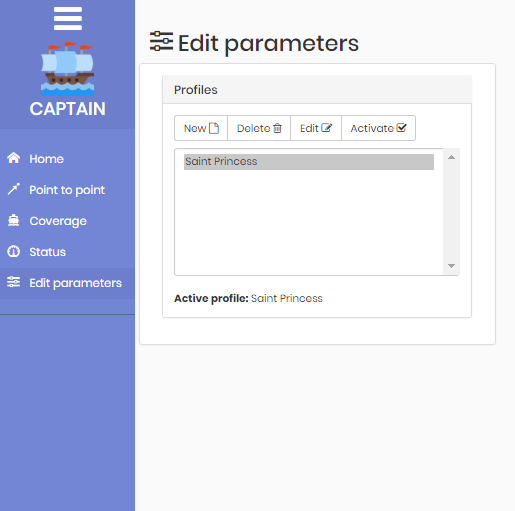
\includegraphics[width=0.9\linewidth]{Images/Implementation/edit_page}
\caption{The Edit parameter page of the website}
\label{fig:editpage}
\end{figure}

\subsubsection{Point to point}

The Point to point page consists of 2 sections one with the coordinates and controls and one with map, this can be seen in figure~\ref{fig:p2ppage}. The map is a leaflet map, but since the website is built with AngularJS, a special leaflet map is one called angular-leaflet-directive\cite{leaflet}. 

For the point to point page, the map need to be able to display a marker of the boat and one for where the user wants the boat to go. Also the website need to be able to draw a path, calculated by the navigation. There for the map is setup with marker that takes the boats boats position, and one that starts out being invisible for the position where the user wants the boat to go. The user can either click the map or, input coordinates directly in the input fields. What ever the user chooses the updateEndCoord function is called, this function show in listing~\ref{lst:updateendcoord}, takes the position inputted. It then assigns it to the marker on the map, since the markers position is data bound to the input fields it automatically update. Also the marker is set to be visible 

\begin{lstlisting}[caption = {updateEndCoord in p2p.js}, captionpos=b, label={lst:updateendcoord}, language=C++,firstnumber=1]
updateEndCoord = function(end_coord) {
        if (end_coord.lat != undefined) {
            $scope.Cached_data_.markers_p2p_[1].lat = end_coord.lat;
        }
        if (end_coord.lng != undefined) {
            $scope.Cached_data_.markers_p2p_[1].lng = end_coord.lng;
        }
        $scope.Cached_data_.markers_p2p_[1].opacity = 1;
    }
\end{lstlisting}

To make sure that the boat position is always up to date, a loop is created from where all other functions are called. This can be seen in listing~\ref{lst:getData}. Every second the function getDataFromNav is called which get the content of the fromNav file which contains the GPS coordinates for the boat, and much more. The boat pose is then updated on the map.

\begin{lstlisting}[caption = {Updating the boat pose in p2p.js}, captionpos=b, label={lst:getData}, language=C++,firstnumber=1]

let main_interval_ = 1000; //The interval for getting new navData

let main_promise = $interval(function() {
        getDataFromNav("../savedData/fromNav.json");
    }, main_interval_); //Update frequency for the boat data

...

getDataFromNav = function(path) {
        return $http.get(path).then(function(response) {
            //Parse fromNav.json, add telemetry data
            updateBoatPose(response.data.Telemetry_);
            $scope.Cached_data_.Path_ = response.data.Path_;
        }).catch(function(data) {
            $scope.Cached_data_.Boat_pose_ = {
                //Default boat position, for testing purposes
                latitude_: 0,
                longitude_: 0,
                orientation_: 0
            };
        });
    }
    
...

updateBoatPose = function(pose) {
        $scope.Cached_data_.Boat_pose_ = pose;
        //Boat marker, set to the boats current position
        $scope.Cached_data_.markers_p2p_[0].lat = pose.latitude_
        $scope.Cached_data_.markers_p2p_[0].lng = pose.longitude_
        $scope.Cached_data_.markers_p2p_[0].iconAngle = pose.orientation_
    }
\end{lstlisting}

When a position on the map has been chosen and boat position is updated. The user can press the "Calculate path" button which call the Action function this function is in charge of change the state of the button as well as sending right task to the navigation. Since this is the first time the User presses the button, it changes it look to reflect that it is calculating, and then function calculatePath is called. This function builds the JSON object that should be send to the navigation, when it has been saved. It calls the function waitForPath, as seen in listing~\ref{lst:calcPath}. In side the waitForPath function an asynchronous loop is setup and constantly getting the data from the navigation. 

\begin{lstlisting}[caption = {calculatePath and waitForPath in p2p.js}, captionpos=b, label={lst:calcPath}, language=C++,firstnumber=1]
calculatePath = function(end_coord) {
        saveToFile("toNav", {
            "func_": "calcP2P",
            "target_position_": {
                latitude_: end_coord.lat,
                longitude_: end_coord.lng
            }
        });
        //Wait for navigation unit to send a new path
        waitForPath();
        //Return when the Path object has been updated by the controller
    }

    waitForPath = function() {
        let current_timestamp = $scope.Cached_data_.Path_.timestamp_;
        $scope.waitForPathPromise = $interval(function() {
            getDataFromNav("../savedData/fromNav.json");
            $http.get("../savedData/fromNav.json").then(function(response) {
                $scope.Cached_data_.Path_ = response.data.Path_;
		if (current_timestamp < $scope.Cached_data_.Path_.timestamp_) {
			$interval.cancel($scope.waitForPathPromise);
                	$scope.Cached_data_.action_state_p2p_ = 1;
		 	setPath(response.data.Path_.line_)
			$scope.Action();
                }
            });
        }, wait_for_path_interval_); //Update frequency for the boat data
    }
\end{lstlisting}

When the waitForPath function get data from the navigation it calls the setPath function, which is show in listing~\ref{lst:setpath}. setPath takes the data from the navigation and displays it on the map as a blue line. After the path is drawn it calls the Action function, which now changes the button state to be start.

\begin{lstlisting}[caption = {setPath in p2p.js}, captionpos=b, label={lst:setpath}, language=C++,firstnumber=1]
setPath = function(path) {
		$scope.Cached_data_.paths_p2p_.p2.latlngs.splice (0,$scope.Cached_data_.paths_p2p_.p2.latlngs.length);
		//Run through all elements in the path and overwrite what is in the paths_ object
		for (let i = 0; i < path.length; i++) {
			$scope.Cached_data_.paths_p2p_.p2.latlngs[i] = {
				lat: path[i].latitude_,
				lng: path[i].longitude_
			}
		}
	}
\end{lstlisting}

When the user presses the start button the Action function is called. The action state dictates that the start function should be called.  The website save a start task in the toNav.JSON file, then it calls the waitForCompletion function, as seen in listing~\ref{lst:start}. Which starts an asynchronous loop that read the data in fromNav.JSON. With this data it updates the progress and ETE, as well as displaying the completed path on the map as a green line. 

\begin{lstlisting}[caption = {the start and waitForCompletion functions in p2p.js}, captionpos=b, label={lst:start}, language=C++,firstnumber=1]
    //Send command to navigation unit
    start = function() {
        saveToFile("toNav", {
            "func_": "start"
        });
        $scope.Cached_data_.ETE_.class_p2p_ = "progress-bar"
        //Wait for navigation unit to send a new path
        waitForCompletion()
        //Return when the path has been traversed
    }

    waitForCompletion = function() {
        $scope.Cached_data_.ETE_.time_p2p_ = "Calculating ...";
        $scope.waitForCompletionPromise = $interval(function() {
            if ($scope.Cached_data_.ETE_.progress_p2p_ >= 100) {
                $scope.Cached_data_.ETE_.time_p2p_ = "Arrived at target";
                $scope.Cached_data_.ETE_.class_p2p_ = "progress-bar-success"
                $scope.Cached_data_.action_state_p2p_ = 3;
                saveToFile("toNav", {
                    "func_": "none"
                });
                $scope.Action()
                $interval.cancel($scope.waitForCompletionPromise);
            } else {
                getDataFromNav("../savedData/fromNav.json");
                $http.get("../savedData/fromNav.json") .then(function(response) {
					$scope.Cached_data_.ETE_.progress_p2p_ = response.data.Progress_.percentage_;
                    $scope.Cached_data_.ETE_.time_p2p_ = response.data.Progress_.ete_;
                    setCompletedPath(response.data.Completed_path_.line_);
                })
            }
        }, wait_for_completion_interval_)
    }
\end{lstlisting}

At any point in time the user can press the "Stop" button which call the Stop function. It sends a stop task to the navigation through the toNav.JSON file, seen in listing~\ref{lst:stop}. Also the Stop function updates some visuals, for example it makes the progress bar red, and makes the ETE say "Canceled".

\begin{lstlisting}[caption = {Stop function in p2p.js}, captionpos=b, label={lst:stop}, language=C++,firstnumber=1]
    $scope.Stop = function() {
            //Reset action state and destroy both waiting promises if they exist
            $scope.Cached_data_.action_state_p2p_ = 0;
            if ($scope.waitForPathPromise) {
                $interval.cancel($scope.waitForPathPromise);
            }
            if ($scope.waitForCompletionPromise) {
                $interval.cancel($scope.waitForCompletionPromise);
            }
            $timeout.cancel($scope.p2ptimeout);
            $scope.Cached_data_.action_p2p_ = {
                text_: "Calculate Path",
                class_: "btn-warning",
                icon_: "glyphicon glyphicon-flash"
            }
    
            //Update command file
            saveToFile("toNav", {
                "func_": "stop"
            });
    
            $scope.Cached_data_.action_state_p2p_ = 0
            $scope.Cached_data_.ETE_.time_p2p_ = "Canceled";
            $scope.Cached_data_.ETE_.class_p2p_ = "progress-bar-danger"
        }
\end{lstlisting}

\subsubsection{Coverage}
Coverage is in many ways the same as point to point, the only real difference is that it uses 2 makers instead of two. Using two makers means that it needs to create a different task to send to the navigation, an example of this creation can be seen in listing~\ref{lst:coveragerectangle}.


\begin{lstlisting}[caption = {CoverageRectangle creation in  coverage.js}, captionpos=b, label={lst:coveragerectangle}, language=C++,firstnumber=1]
calculatePath = function(end_coord) {
        saveToFile("toNav", {
            "func_": "calcP2P",
            "target_position_": {
                latitude_: end_coord.lat,
                longitude_: end_coord.lng
            }
        });
        //Wait for navigation unit to send a new path
        waitForPath();
        //Return when the Path object has been updated by the controller
    }
\end{lstlisting}

The visual design is also almost the same as point to point, but as explained there are two points. The coverage map represent the two markers with some similar looking ones, where they are labeled 1 and 2. The labeling is to indicate where the boat is going to start and end. In figure~\ref{fig:coveragepage}, a orange rectangle is also highlighting the area that has been covered by the points. 

\begin{figure}[H]
\centering
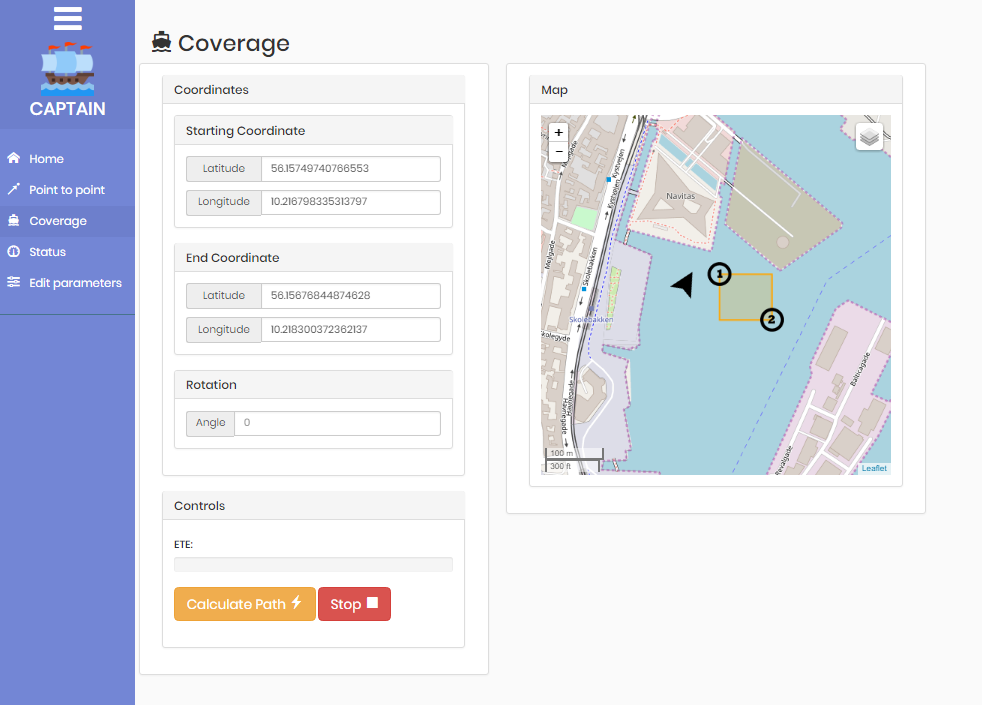
\includegraphics[width=0.9\linewidth]{Images/Implementation/coverage_page}
\caption{Visual design of the coverage page}
\label{fig:coveragepage}
\end{figure}


\subsubsection{Status}
The status page is used to display diagnostics data. The diagnostics data comes from the navigation part of the system, where gps data and motor status' are handles. The status page is implemented to specify the exact data it wants to display, but instead dynamically read from the fromNav.JSON file. In this file there is a javascript list named \texttt{Status\_} which holds any amount of generic status objects. This protocol is described in detail in section ~\ref{sec:protocol_fromNav} on page ~\pageref{sec:protocol_fromNav}. Because this javascript list can hold any number of objects, the status page can display any number of items. 

To display all of the status messages, it need somewhere to put it, there for in the HTML of the page a \texttt{<div>} tag is data bound to a variable. If the variable contains HTML it will get displayed, the HTML syntax can be seen in listing~\ref{lst:statushtml}.

\begin{lstlisting}[caption = {Html for displaying status'}, captionpos=b, label={lst:statushtml}, language=C++,firstnumber=1]
<div class="col-lg-5 col-md-offset-025 panel panel-default">
 <div class="panel-body">
     <div ng-bind-html="Status_panels_">
     </div>
		<div class="panel panel-default">
         <div class="panel-heading">
             <h3 class="panel-title">Update</h3>
         </div>
         <div class="panel-body">
             <div class="alert" ng-class="Time_since_last_data_.warning_" style=" display:inline-block; padding-top=1em">
                 <strong>Info:</strong> Time since last status message: {{Time_since_last_data_.time_}} s<br />
             </div>
         </div>
     </div>
 </div>
</div>
\end{lstlisting}

When the data from the fromNav.JSON file has been loaded, the updateStatusDisplay function is called with the javascript list \texttt{Status_}, and the timestamp of when the fromNav.JSON file was created. As it can be seen in listing~\ref{lst:statusjs}, the code runs through all of the status items, and takes the relevant data, and encloses it in the necessary HTML. When the HTML is built for all of \texttt{Status_} it is assigned to the \texttt{div} tag from the html. It is important to notice that the code explicitly tells Angular that it can trust the HTML just created as HTML. This has to be done to tell Angular that we are sure that cross site scripting isn't possible with this HTML. 

\begin{lstlisting}[caption = {displaying status messages }, captionpos=b, label={lst:statusjs}, language=C++,firstnumber=1]
updateStatusDisplay = function(status, timestamp) {
        let html = ""; //Creates a variable containing the html
        status.forEach(function(current_value) {
			//For each status object it creates a panel with the necessary data
            html += `
      <div class="panel panel-default">
      	<div class="panel-heading">
      		<h3 class="panel-title">` + current_value.title_ + `</h3>
      		</div>
      		<div class="panel-body">`;

            current_value.items_.forEach(function(item) {
                html += "<strong>" + item.title_ + ":</strong> " + item.data_ + " " + item.unit_ + "<br />"
                if (item.unit_ == '%') {
                    html += `<div class="progress">
                  			<div class="progress-bar ` + item.color_ + `  " role="progressbar" aria-valuenow="0" aria-valuemin="0" aria-valuemax="100" style="width: ` + item.data_ + `%">
                  			</div>
                  		</div>`;
                }
            });

			//Adds ending html
            html += `
      		</div>
      	</div>
      </div>`
        })
        $scope.Status_panels_ = $sce.trustAsHtml(html); //Sets the panels to the html created and trusts it, maybe not good for security

		//Updates the time size last data panel.
        $scope.Time_since_last_data_.time_ = Math.round((Date.now() - timestamp) / 1000);
        if ($scope.Time_since_last_data_.time_ > 20) {
            $scope.Time_since_last_data_.warning_ = "alert-danger";
        } else if ($scope.Time_since_last_data_.time_ > 10) {
            $scope.Time_since_last_data_.warning_ = "alert-warning";
        } else {
            $scope.Time_since_last_data_.warning_ = "alert-info";
        }


    };
\end{lstlisting}

The status page also has a Map just like the point to point page and coverage page. On the status page, only the boat position is displayed. The final visual design of the status page can be seen in figure~\ref{fig:statuspage}. It is some example diagnostics data, which is very like the data got from the navigation.

\begin{figure}[H]
\centering
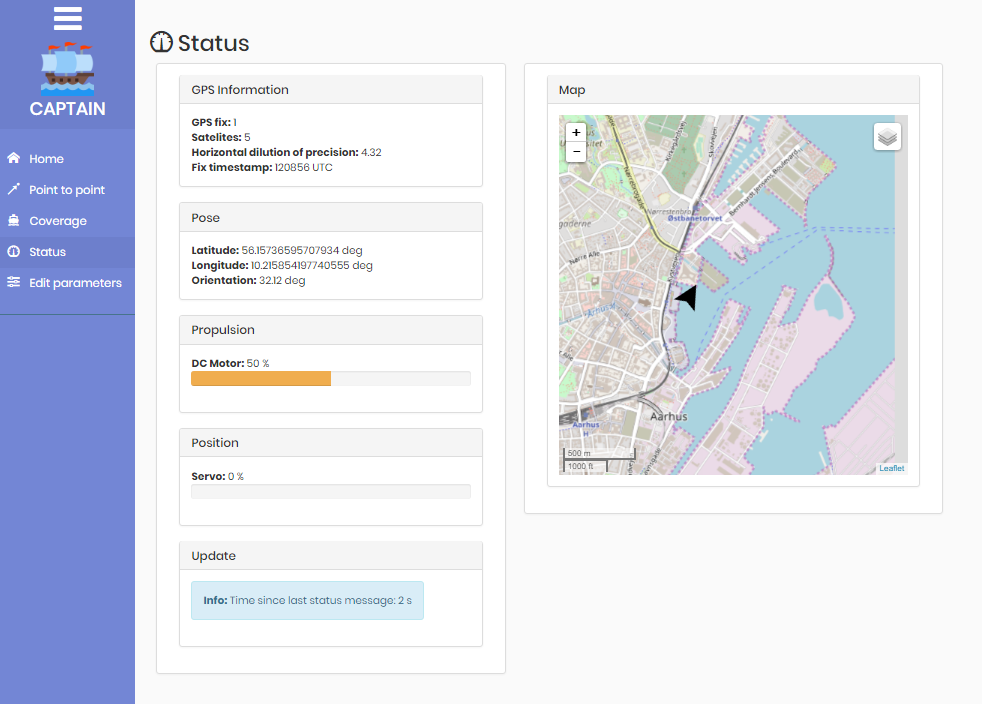
\includegraphics[width=0.7\linewidth]{Images/Implementation/status_page}
\caption{Visual design for displaying diagnostics data on the status page}
\label{fig:statuspage}
\end{figure}


\subsection{Nodejs server}
\label{sec:nodejs_server}
The Nodejs server can be thought of as the back-end of the website, it is what needs to run for the website to be live. Nodejs is a javascript runtime\cite{nodejs}. This project uses the server to handle three of post calls that the client can make through the website, and also hosting the website on port 80. 

When a post call comes from the client with either a "/profiles", "/active" or "/toNav" url, the server takes the data it gets and writes it to the appropriate file, lets take "/profiles" as an example, The node package fs, is used to save the data to the profiles.json file in the savedData folder in the website, as seen in listing~\ref{lst:post}. After the file is saved then it returns a status 200, if it did not work it returns a status 500, which is a server error.

\begin{lstlisting}[caption = {Handeling a POST call to url "/profiles"}, captionpos=b, label={lst:post}, language=C++,firstnumber=1]
app.post('/profiles',function(req, res){
	console.log(req.body);
	res.set("Connection", "close");
	res.setHeader('Content-Type', 'application/json');

	fs.writeFile(website_path+'/savedData/profiles.json', JSON.stringify(req.body), function(err) {
	    if(err) {
			res.sendStatus(500);
	        return console.log(err);
	    }
	});
	res.sendStatus(200);

});
\end{lstlisting}

To host the website, the server is listening for a client, and if one connects the server, serves the client with the website. This can be seen in listing~\ref{lst:host}.

\begin{lstlisting}[caption = {Hosting server}, captionpos=b, label={lst:host}, language=C++,firstnumber=1]
app.use(express.static(website_path))

...

//wait for a connection
app.listen(80, function () {
  console.log('Server is running. Point your browser to: '+ip.address()+':80');
});
\end{lstlisting}

